In 1980, Robert Plutchik proposed a psychoevolutionary classification approach for general emotional responses. He considered there to be eight primary emotions—anger, fear, sadness, disgust, surprise, anticipation, trust, and joy. He also discussed about the bipolar relationship between them and created a two dimensional wheel model to illustrate different emotions which is known as the Plutchik's Wheel of Emotions as shown in figure \ref{Fig:fig3}.

\begin{figure}[H]
	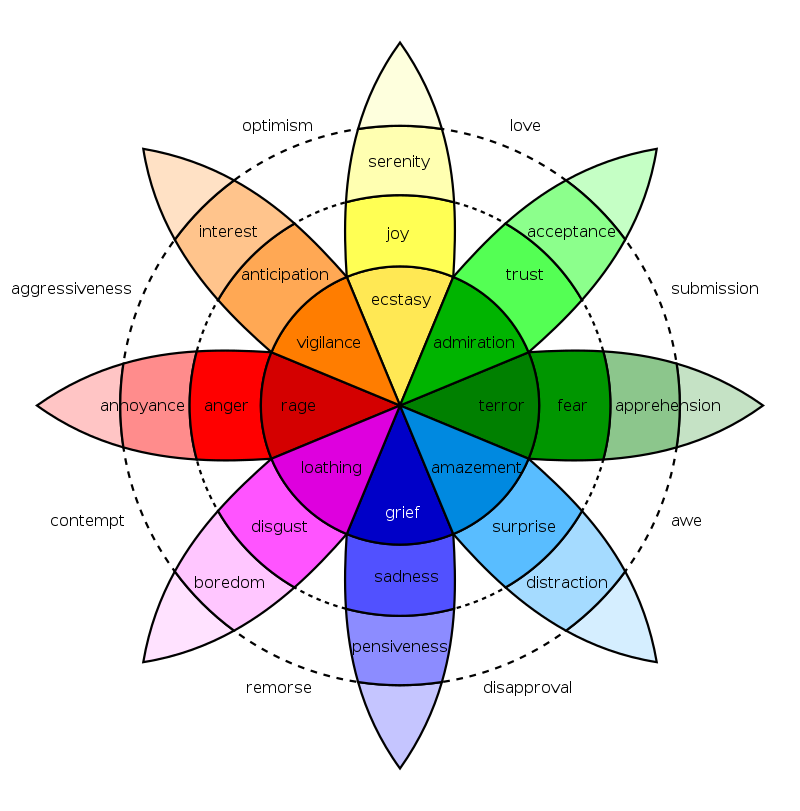
\includegraphics[width=\columnwidth, keepaspectratio]{Plutchik'sWheelofEmotions}
	\caption{Plutchik's Wheel of Emotions}
	\label{Fig:fig3}
\end{figure}

According to Plutchik, the petals which are opposite to each other in this 2D represiontation, represents the bipolar or opposite emotion. For example, anger is opposite to fear, grief is opposite to ecstacy, and so on. Some emotions are made by the combination or addition of the emotions represented by the two adjacent leaves of this wheel. For example, love is the addition of joy and trust, optimism is created by the combination of anticipation and joy. Also, the intensity of emotions will increase as we go towards the center of this wheel and vice versa\cite{enwiki:1136521972}.